\chapter{Detailed Implementation}
\label{chap:detailed-implementation}

This chapter summarizes the implementation details of the Zero-Knowledge Logistic Regression (ZKLR) system. The design integrates machine learning computation, zero-knowledge circuits, and cryptographic proof generation into a coherent workflow that demonstrates practical privacy-preserving inference. The implementation focuses on correctness, reproducibility, and computational efficiency while maintaining modularity for future extensions.

% =====================================================================
\section{System Architecture}
% =====================================================================

\subsection{Overview}

The ZKLR system adopts a modular architecture separating dataset preparation, model training, proof generation, verification, and performance evaluation. This design aligns with modern ZKP workflow practices that separate circuit compilation, witness generation, and proof verification. The data layer generates a synthetic dataset and trains a logistic regression model under controlled conditions. The proof-generation layer transforms inputs into witness assignments and constructs PLONK proofs demonstrating correct model inference without revealing private values, following the zero-knowledge definition introduced by Goldwasser et al.. Verification validates these proofs efficiently, and a metrics layer collects runtime statistics and visualizes performance behaviour.

\subsection{Technology Stack}

The implementation combines Python for numerical computation and Go for proof generation. Go 1.24.1 supports the gnark framework (v0.11.0), implementing PLONK-style proof systems as described by Kates et al.. Python 3.8+ facilitates dataset generation, logistic regression training, and plotting. The hybrid design leverages Python's machine learning ecosystem while ensuring performance and type safety during cryptographic operations.

% =====================================================================
\section{Dataset Handling}
% =====================================================================

\subsection{Dataset Overview}

A synthetic dataset containing 3,000 samples forms the evaluation baseline. Each record consists of a single numerical feature representing student marks from 0 to 100, accompanied by binary pass–fail labels. The reproducibility of the dataset is ensured through fixed random seeds, following standard practices in logistic regression modeling.

\subsection{Dataset Generation and Training}

The dataset is generated using uniform sampling followed by rule-based labeling, with added noise to prevent deterministic separation. Logistic regression is trained using scikit-learn with default parameters. The learned weights and bias are exported and encoded into fixed-point representations suitable for arithmetic circuits, bridging the floating-point domain with finite-field computation.

% =====================================================================
\section{Model Design}
% =====================================================================

\subsection{Logistic Regression Formulation}

Logistic regression estimates probabilities by evaluating the linear function
\begin{equation}
    z = wx + b
\end{equation}
and applying the sigmoid function
\begin{equation}
    \sigma(z) = \frac{1}{1 + e^{-z}},
\end{equation}
as defined in classical statistical modeling literature. The model’s simplicity and numerical stability make it suitable for zero-knowledge circuit construction, where each operation must be represented using finite-field arithmetic.

\subsection{Fixed-Point Encoding}

Since finite-field arithmetic does not natively support floating-point operations, values are encoded using fixed-point formats. In this representation, a value is stored as an integer scaled by a fixed power of two, where the format Qm denotes m fractional bits of precision. The system uses Q32 (32 fractional bits) for intermediate linear computations, Q10 (10 fractional bits) for indexing logits into the sigmoid lookup table, and Q16 (16 fractional bits) for final outputs. This multi-precision strategy balances accuracy and computational cost, ensuring numerical stability and preventing overflow, consistent with principles from ZKP arithmetic circuit design.

% =====================================================================
\section{Circuit Construction}
% =====================================================================

The circuit verifies that the predicted label corresponds to a valid logistic regression inference without revealing private model weights or intermediate values. Its structure ensures completeness, soundness, and zero-knowledge as established in.

\subsection{Circuit Configurations and System Parameters}

\begin{figure}[h]
    \centering
    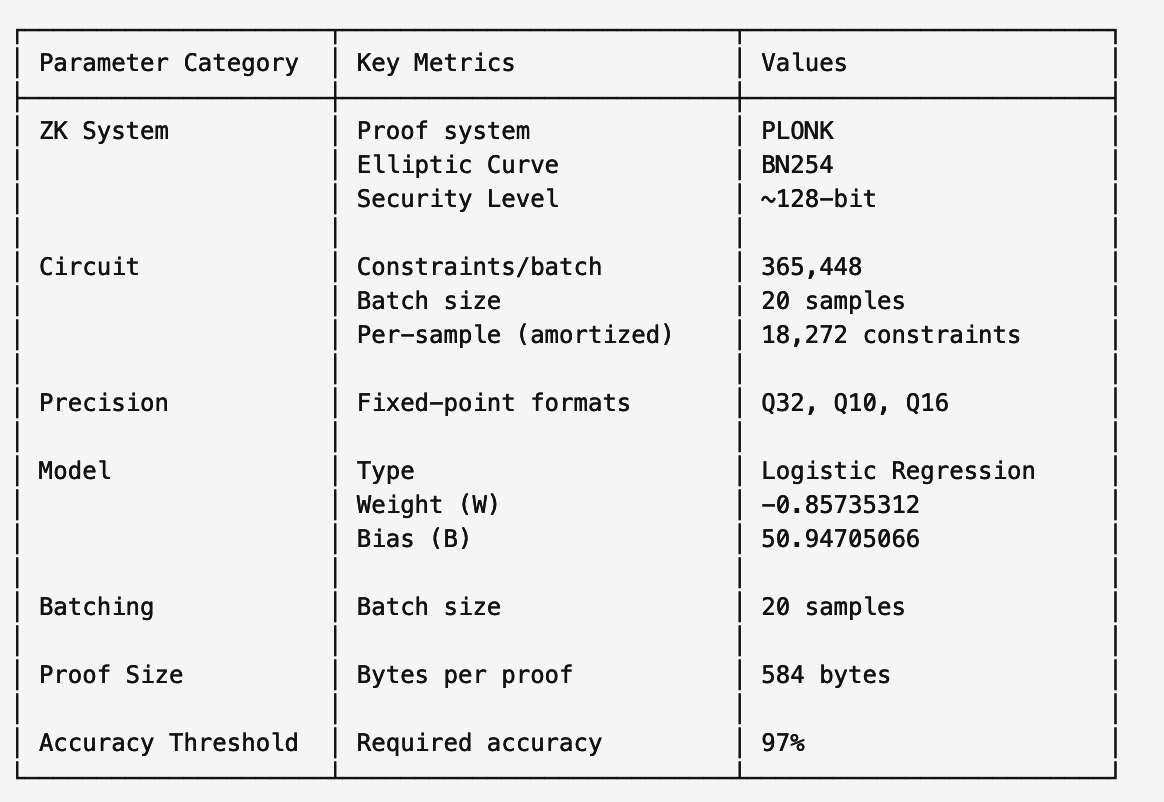
\includegraphics[width=0.75\textwidth]{congifs_invert.png}
    \caption{Configurations for the circuit}
    \label{fig:configuration}
\end{figure}

This image summarizes the core configuration parameters used in the zero-knowledge logistic regression system. These parameters define the circuit’s structure, numerical precision, proof characteristics, and batching strategy adopted during proof generation. The configuration reflects a trade-off between computational efficiency and verification soundness, ensuring both practical performance and strong cryptographic guarantees.

\subsection{Circuit Layers}

The sigmoid function is implemented using a lookup table of 8,192 precomputed values. This avoids evaluating exponentials inside the circuit, consistent with efficiency practices in ZKP systems. Symmetry is used to halve storage requirements via the identity 

\begin{equation}
    \sigma(-z) = 1 - \sigma(|z|),
\end{equation}

ensuring correctness within the finite-field framework. The final computation binds the predicted label to the claimed output, enforcing soundness.

\subsection{Circuit Algorithm}
The circuit algorithm defines the constraints required to verify logistic regression inference within the zero-knowledge framework. It encodes both the linear computation and the non-linear sigmoid transformation as arithmetic operations over a finite field.

\begin{figure}[h]
    \centering
    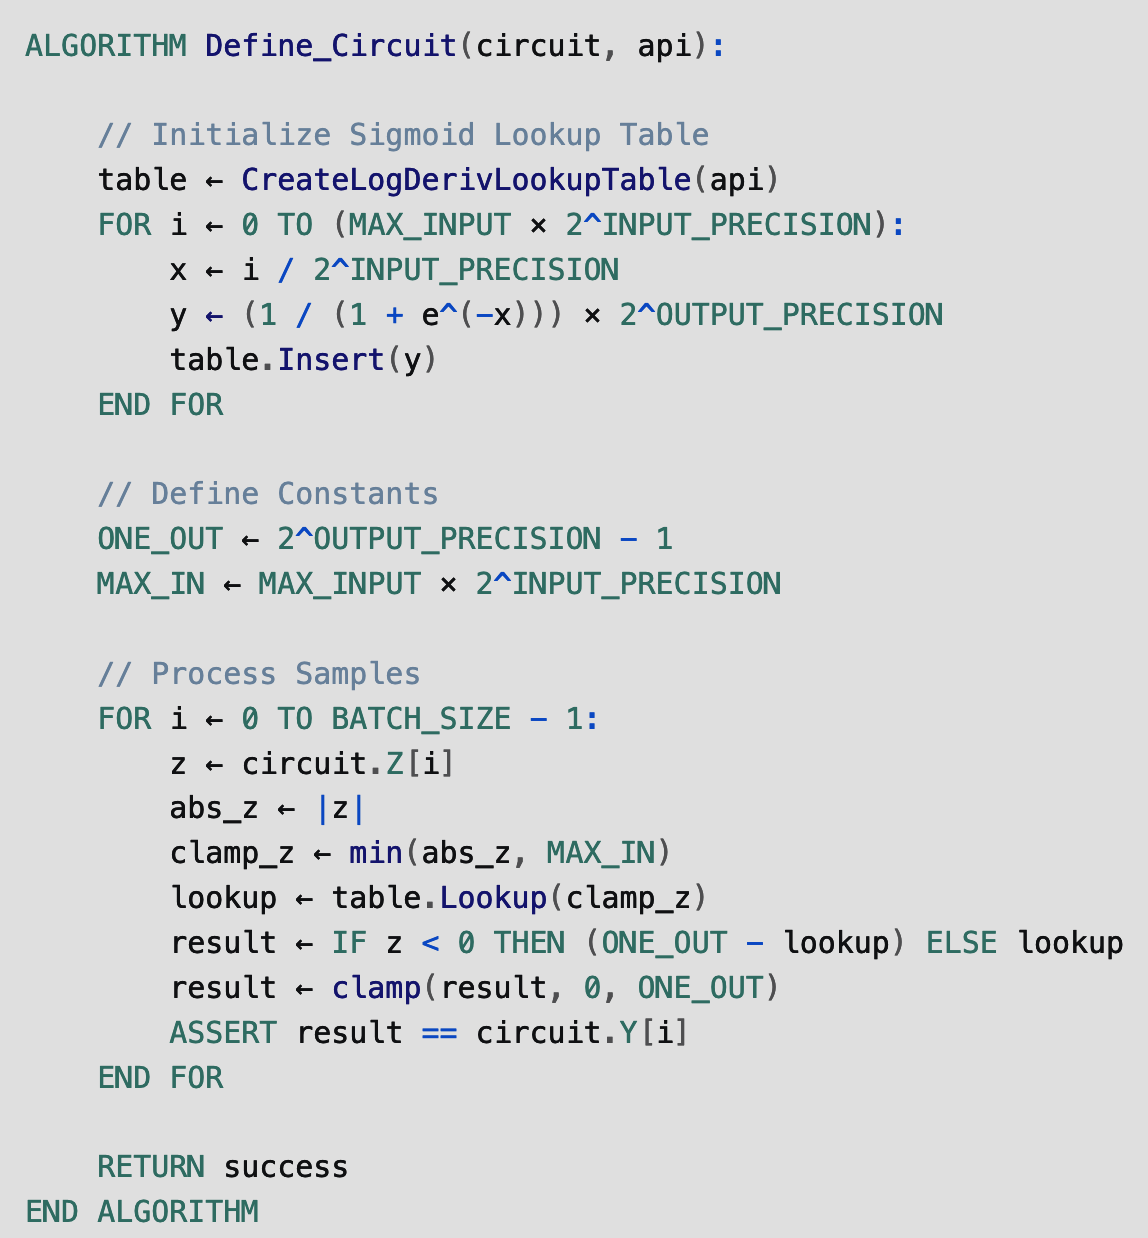
\includegraphics[width=0.75\textwidth]{image (2).png}
    \caption{Pseudocode for Circuit Algorithm}
    \label{fig:algorithm}
\end{figure}

This algorithm captures the full inference pipeline of logistic regression within an arithmetic circuit. By representing each operation as a verifiable constraint, it ensures that the prover can only produce valid proofs corresponding to genuine model computations, thus preserving soundness and correctness under zero-knowledge guarantees.

\subsection{Constraint Count}

The optimized circuit contains 58,028 constraints. Lookup-table enforcement forms the majority of these constraints, reflecting the complexity inherent in embedding non-linear functions into arithmetic circuits. Remaining constraints ensure correctness of sign handling, linear computation, and output binding.

\subsection{Constraint Design}
The arithmetic circuit enforces the correctness of the logistic regression inference through a layered set of constraints. Each constraint corresponds to a verifiable algebraic relationship that ensures the model’s output is consistent with the claimed computation.

\begin{figure}[H]
    \centering
    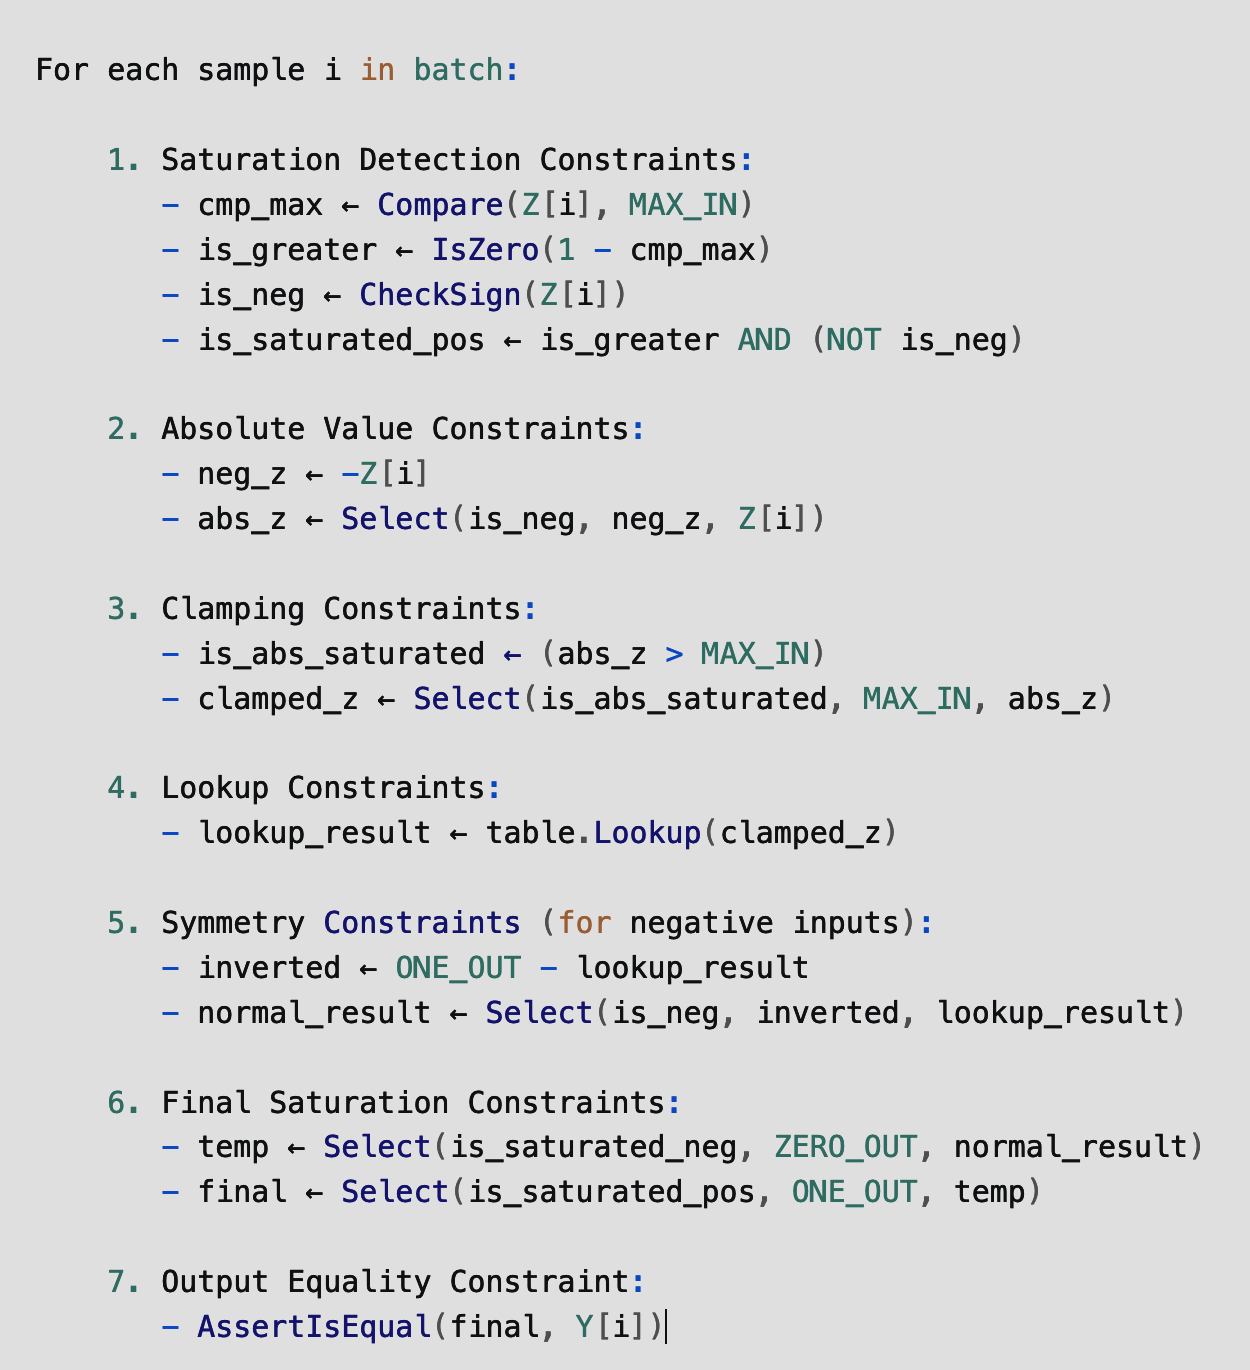
\includegraphics[width=0.75\textwidth]{constraints.png}
    \caption{Constraints in Arithmetic Circuits}
    \label{fig:constraints}
\end{figure}

Together, these constraints ensure that the circuit remains sound, complete, and consistent with the logistic regression inference function, while adhering to the zero-knowledge property.

% =====================================================================
\section{Proof Generation Workflow}
% =====================================================================

\subsection{Setup Phase}

Proof generation starts with compiling the circuit  and generating keys for the prover and verifier using the PLONK protocol. This setup step is performed once per circuit and remains constant regardless of dataset size.

\begin{figure}[h]
    \centering
    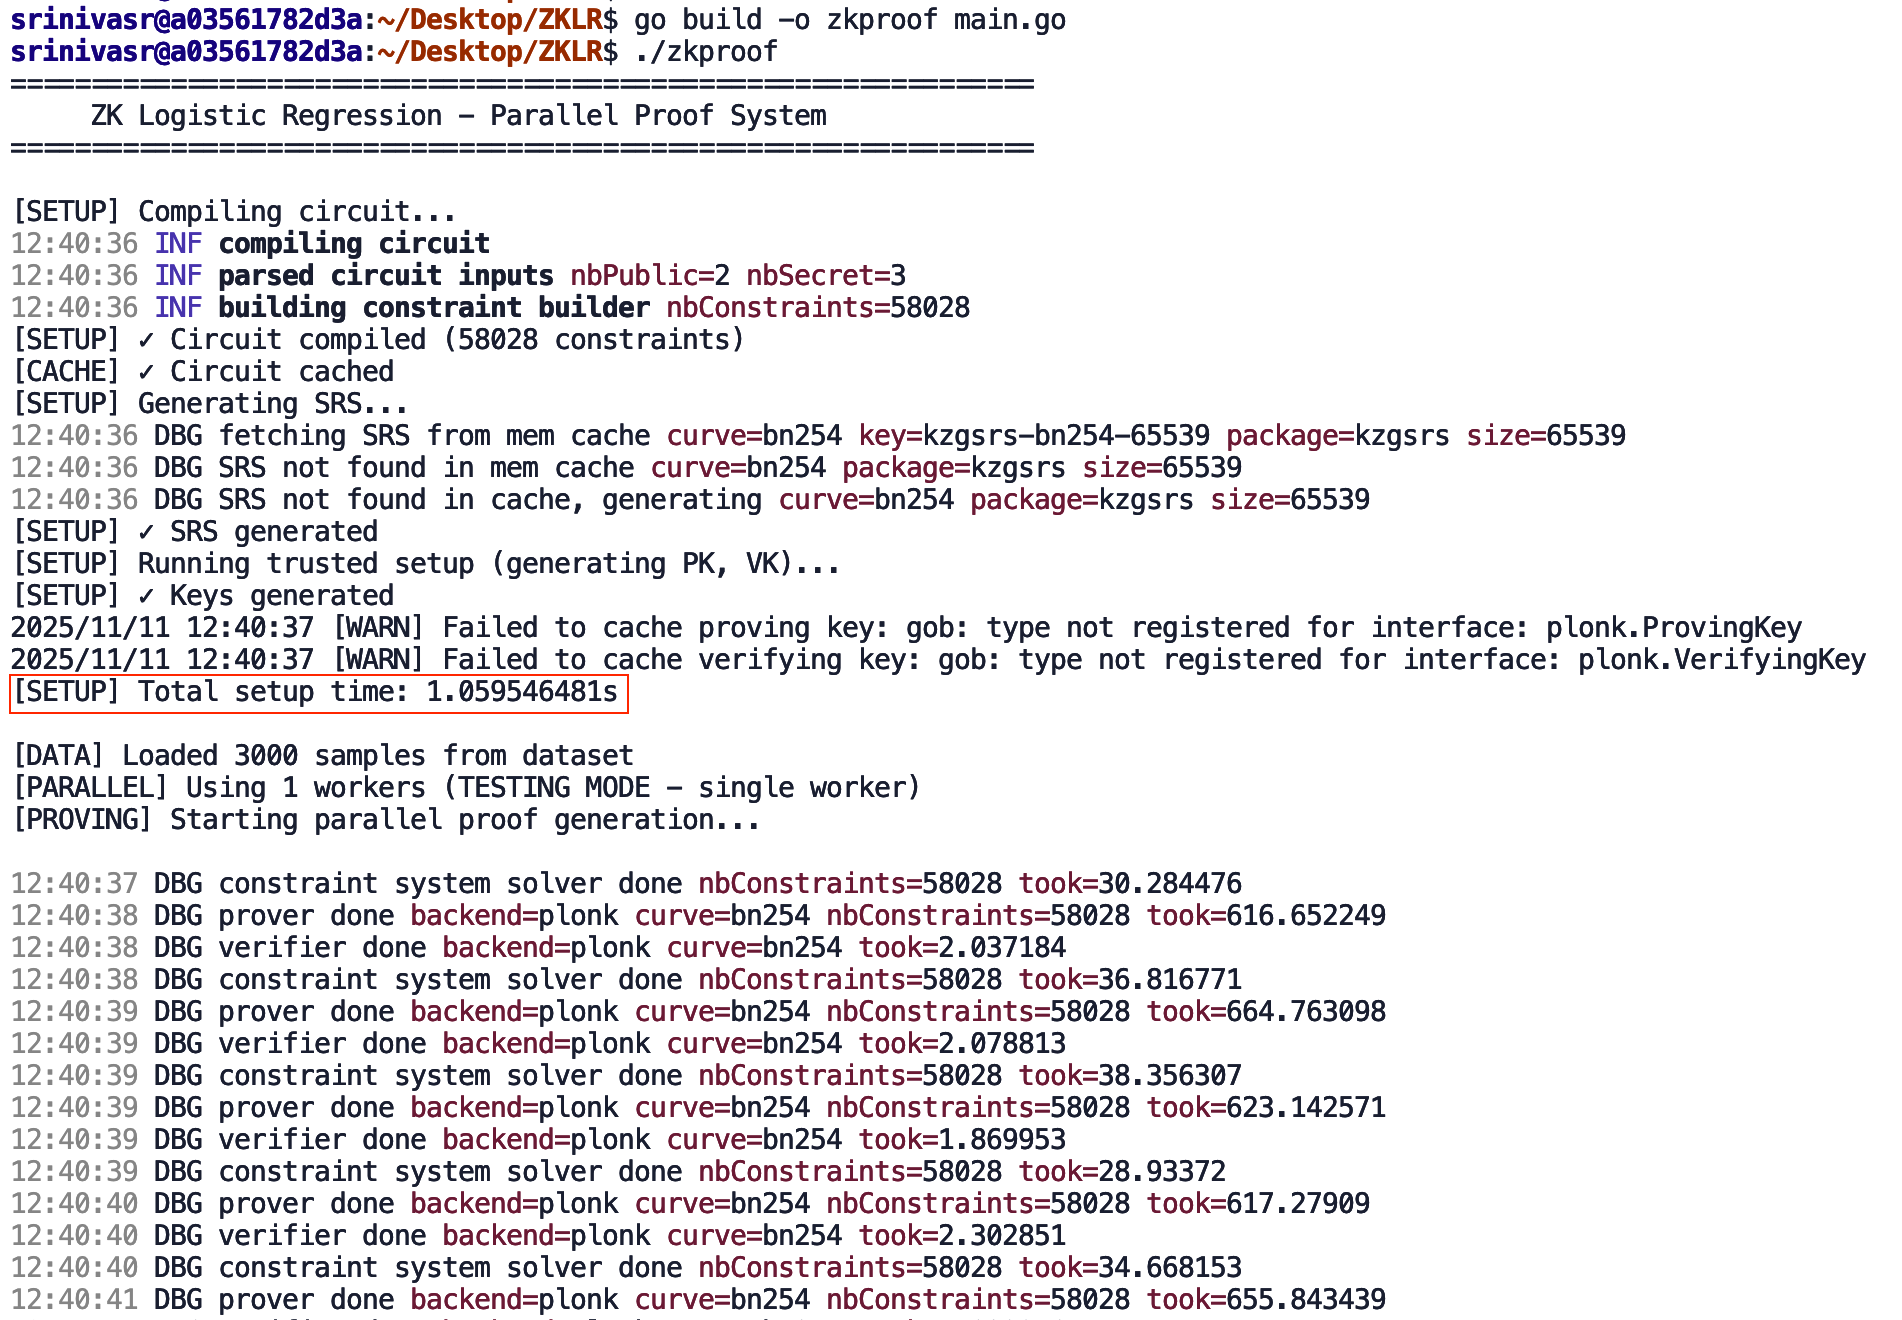
\includegraphics[width=0.75\textwidth]{image.png}
    \caption{Setup time for a circuit}
    \label{fig:setup_time}
\end{figure}

\subsection{Individual Proof Generation}

For each input sample, the system computes the linear score and sigmoid output using fixed-point arithmetic. These values populate the private witness required for proof generation. The size of each PLONK proof is 584 bytes which is in line with the succinctness guarantee of the polynomial commitment scheme.

\begin{figure}[h]
    \centering
    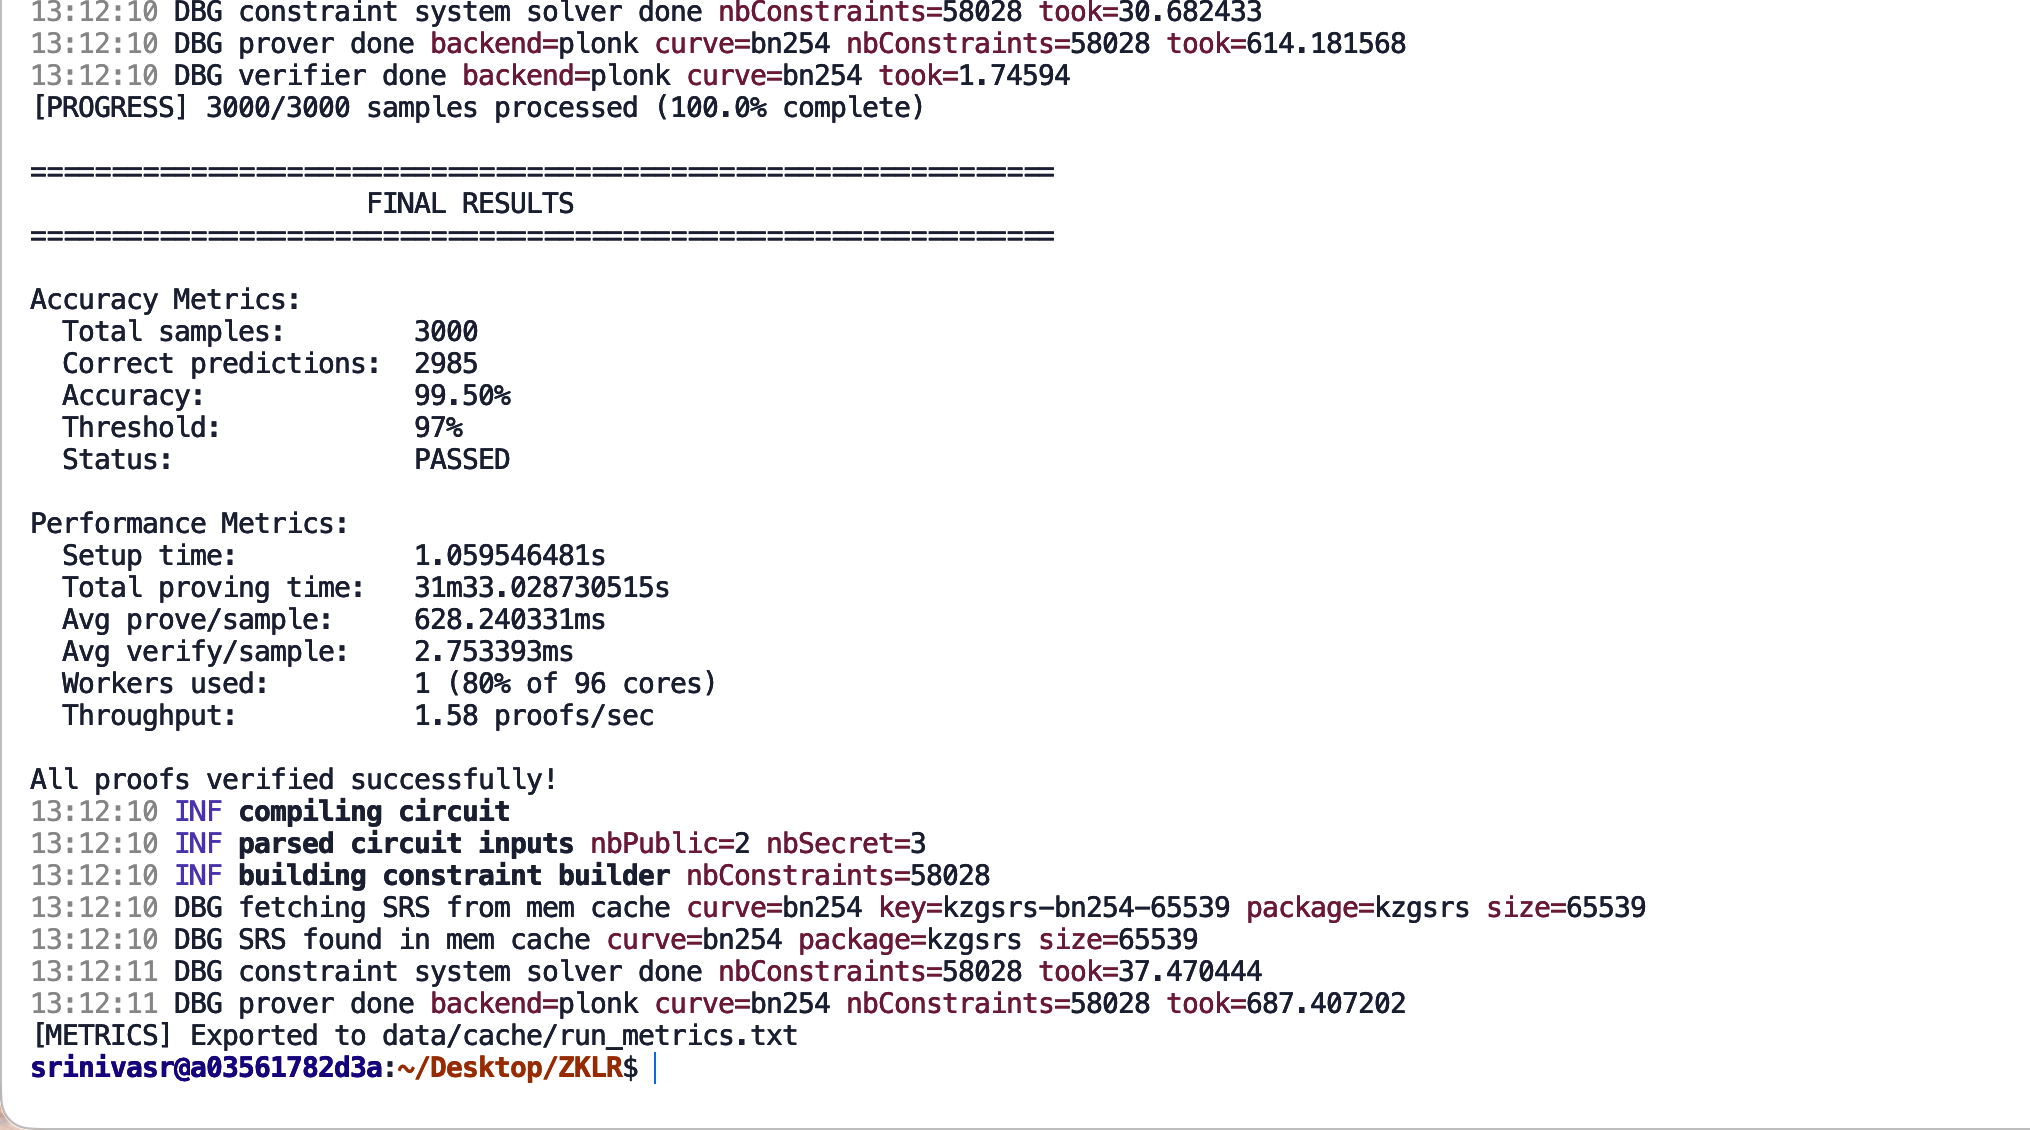
\includegraphics[width=0.75\textwidth]{3.png}
    \caption{Proof generation and verification for individual samples}
    \label{fig:sample_proof_time}
\end{figure}

Verifier validates the proof using the verification key and public inputs only, ensuring zero-knowledge properties as originally defined.

\subsection{Batched Proof Implementation}

Batch proving allows proofs to be generated for multiple samples within a single circuit instance. With 20 samples per batch, the circuit grows to 365,448 constraints but achieves sublinear scaling by reusing setup and lookup-table loading across samples.

\begin{figure}[H]
    \centering
    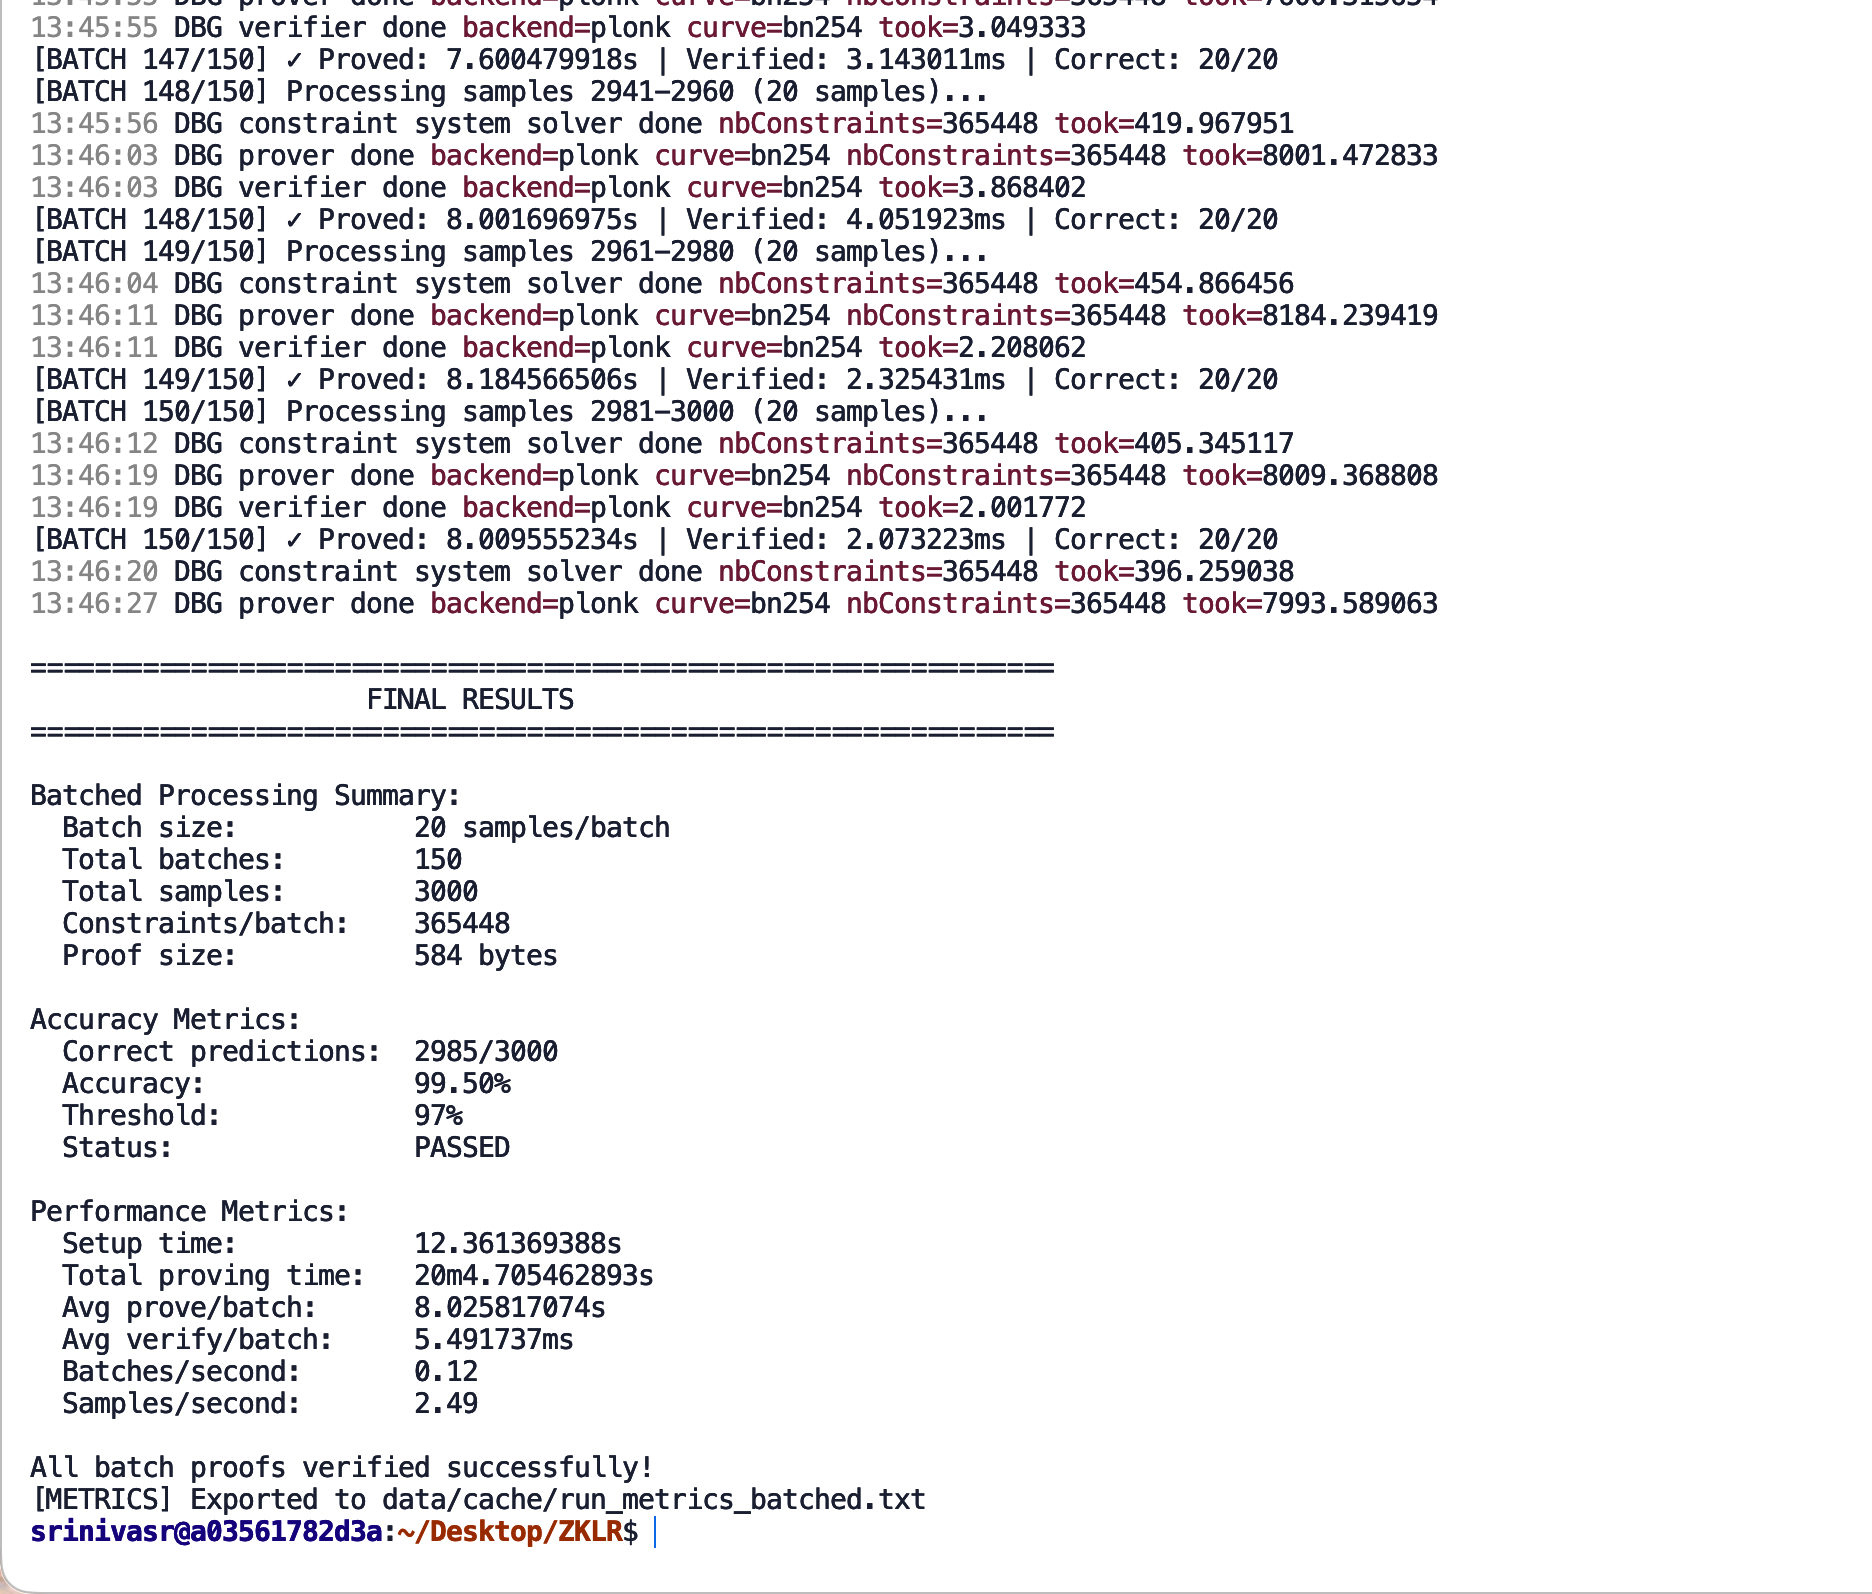
\includegraphics[width=0.75\textwidth]{5.png}
    \caption{Evaluation Metrics for Batched Proofs}
    \label{fig:batched_proof_time}
\end{figure}

% =====================================================================
\section{Performance Optimizations}
% =====================================================================

\subsection{Lookup Table Reduction}

Empirical analysis showed that logits predominantly fall within $[-8,8]$. Restricting the lookup table to this domain reduces entries from 30,720 to 8,192 thus lowering the constraint count and improving proving time by approximately 4.4 times.

\begin{figure}[H]
    \centering
    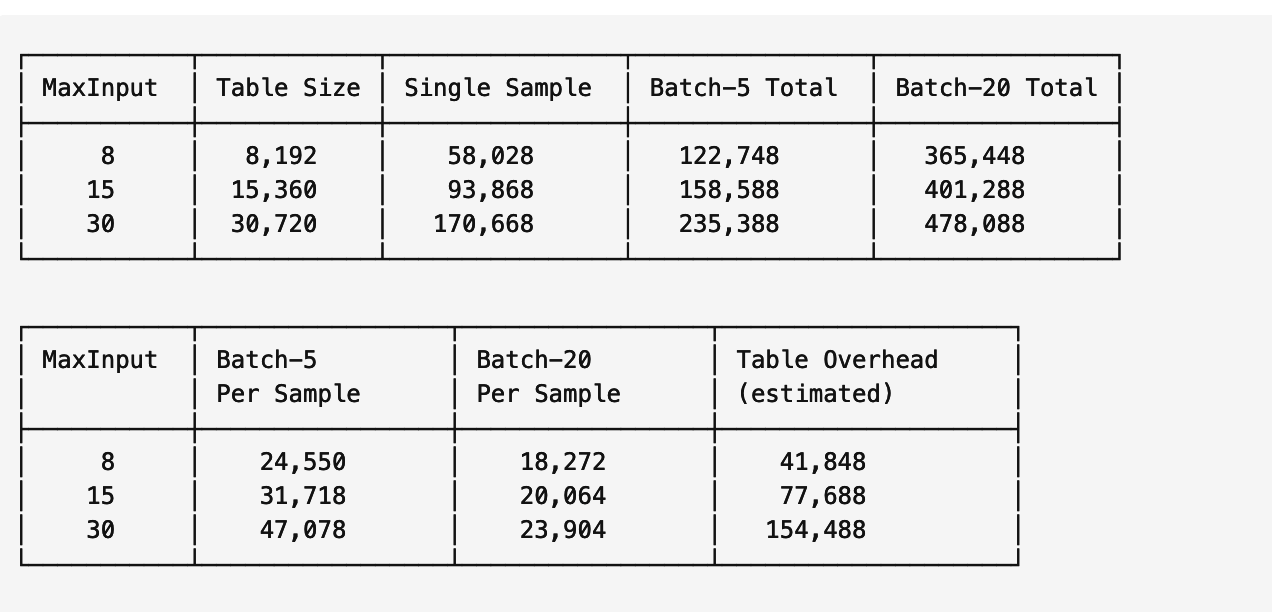
\includegraphics[width=0.75\textwidth]{image (3).png}
    \caption{Lookup Table for Non-linear function}
    \label{fig:lookup_table}
\end{figure}

\subsection{Circuit Caching and Precision Control}

Caching compiled circuits helps avoid repeated preprocessing. Controlled precision preserves numerical stability while minimizing constraint usage, aligning with modern practices in efficient ZK circuit optimization.

% =====================================================================
\section{Security Considerations}
% =====================================================================

The PLONK protocol provides zero-knowledge guarantees consistent with the foundational definition. Soundness relies on the hardness of the discrete logarithm problem over the BN254 elliptic curve, offering approximately 128-bit security. Although this prototype uses a single-party structured reference string (SRS), production environments require multi-party ceremonies to prevent toxic waste retention.

% =====================================================================
\section{Summary}
% =====================================================================

The implementation demonstrates feasible and efficient zero-knowledge verification of logistic regression. The architecture integrates machine learning computation with fixed-point encoding, lookup-table optimization, and cryptographic proof generation. This design ensures strong privacy, predictable runtime behaviour, and accurate classification results, forming a robust foundation for future exploration of zero-knowledge machine learning frameworks.
